\newpage
\section{HJM and LMM}
\subsection{HJM Framework}
\subsubsection{No Arbitrage Condition}
A key things to remember is that {\color{red}all CIR process, Vasicek process are Markov models, and lies in the HJM framework}.
\begin{equation}
\begin{aligned}
f(t, T) - f(0, T) =  \int_0^t (\alpha(u, T)du + \sigma(u, T)) dW(u)
\end{aligned}
\end{equation}

At time t, since the zero bond $B(t, T)$ is a martingale.
 \begin{equation}
\begin{aligned}
log(B(t, T))) &= -\int_t^Tf(t, u)\\
\end{aligned}
\end{equation}

 \begin{equation}
\begin{aligned}
dlog(B(t, T))) &= f(t, t)dt - (\int_t^T \alpha(t, u) du)dt +\int_t^T \sigma(t, u) dW(t) \\
                     &= (f(t, t) - \alpha^\ast(t))dt + \sigma^\ast(t) dW(t)
\end{aligned}
\end{equation}
Then we have
 \begin{equation}
\begin{aligned}
d(B(t, T))) &= f(t, t)dt - (\int_t^T \alpha(t, u) du)dt +\int_t^T \sigma(t, u) dW(t) \\
                     &=B(t, T) (f(t, t) - \alpha^\ast(t) + \frac{1}{2} {\sigma^\ast}^2(t)) dt - \sigma^\ast(t) dW(t)
\end{aligned}
\end{equation}

Then we have

\begin{equation}
\begin{aligned}
d(D(t)B(t, T))) &= f(t, t)dt - (\int_t^T \alpha(t, u) du)dt +\int_t^T \sigma(t, u) dW(t) \\
                     &=D(t)B(t, T) (-\alpha^\ast(t) + \frac{1}{2} {\sigma^\ast}^2(t)) dt - \sigma^\ast(t) d\widetilde{W}(t)
\end{aligned}
\end{equation}

So we need to have
\begin{equation}
\begin{aligned}
 (-\alpha^\ast(t, T) + \frac{1}{2} {\sigma^\ast}^2(t, T)) = \Theta(t) | for T \in [0, T]
\end{aligned}
\end{equation}

Then take derivative with T, we get
\begin{equation}
\begin{aligned}
 \alpha(t, T) = \sigma^\ast(t) \sigma(t, T)
\end{aligned}
\end{equation}

\subsubsection{Some Important Feature}
Once we get no-arbitrage condition, we can have several important conclusion.

First, the T measure under this is vs risk neutral measure.
\begin{equation}
\begin{aligned}
 d\widetilde{W}^T(t) - \sigma^\ast(t) =   d\widetilde{W}(t)
\end{aligned}
\end{equation}

Second, The forward rate's drift is. {\color{red}This means the forward rate can be solely determined by sigma process.}
\begin{equation}
\begin{aligned}
f(t, T) - f(0, T) =  \int_0^t (\sigma^\ast(u) \sigma(u, T)du + \sigma(u, T) dW(u))
\end{aligned}
\end{equation}

\subsection{LMM Framework}
\subsubsection{Forward Payment Replicate}
The first things to remember is how to replicate a pay off for a FRA that pays $L(T, T)$ at time $T + \delta$.
In fact we can {\color{red}have portfolio of $\frac{1}{\delta}B(t, T) - \frac{1}{\delta}B(t, T+\delta)$ to exactly replicate the payoff}.(At time T we need to reinvest our earning of first leg to  $B(T, T+\delta)$ and have payoff  $\frac{1}{\delta B(T, T+\delta)}$)

In fact, the red part is  $B(t, T+\delta) L(t, T)$ and we can think of it as a $T + \delta$ bond times forward rate

\subsubsection{$B(t, T+\delta)$ Measure Pricing Example (T measure)}
Since  $B(t, T+\delta) L(t, T)$ is a price of contract (tradable), so under $B(t, T+\delta)$ measure $L(t, T)$ is a martingale. So for example the price of caplet paying $(L(T, T) - K)^+$ at time $T + \delta$ can be valued as
\begin{equation}
\begin{aligned}
C(t, T) &=  B(t, T+\delta) E^{T+\delta} (L(T, T) - K)^+
\end{aligned}
\end{equation}

Since at  $B(t, T+\delta) L(t, T)$  measure the $L(t, T)$ satisfy $d(L(t, T)) = \gamma(t, T) L(t, T) d\widetilde{W}^{T+\delta}(t)$. {\color{blue}Same as HJM, we need to find a vol process for $L(t, T)$ to price the caplet using blacks formula}

In fact, we can get the $\gamma(t, T)$ by using zero bond at risk neutral measure. Since $F(t, T) = (\frac{1}{\delta}B(t, T) - \frac{1}{\delta}B(t, T+\delta)) / B(t, T+\delta)$

So  we have
\begin{equation}
\begin{aligned}
 F(t, T) + \frac{1}{\delta} &= \frac{B(t, T)}{B(t, T+\delta)}\\
&= \frac{B(0, t)}{B(0, T)} \exp(\int_{0}^{t} (\sigma^\ast(t, T) - \sigma^\ast(t, T+\delta)) \cdot d\widetilde{W}(u) \\ &-0.5\int_{0} ^ {t} \norm{\sigma^\ast(t, T) - \sigma^\ast(t, T+\delta)} ^ 2 du \\
&- \int_0^t\sum_{1} ^ {d} \sigma^\ast_{i}(t, T+\delta)(\sigma^\ast_{i}(t, T) - \sigma^\ast_{i}(t, T+\delta) du)
\end{aligned}
\end{equation}

So
\begin{equation}
\begin{aligned}
 d(F(t, T)) &= (F(t, T) + \frac{1}{\delta}) \\
 &-  (\sum_{1} ^ {d}  \sigma^\ast_{i}(t, T+\delta)(\sigma^\ast_{i}(t, T) - \sigma^\ast_{i}(t, T+\delta) du +  (\sigma^\ast(t, T) - \sigma^\ast(t, T+\delta)) \cdot d\widetilde{W}(u)) \\
 &= (F(t, T) + \frac{1}{\delta}) (\sigma^\ast(t, T) - \sigma^\ast(t, T+\delta)) \cdot d\widetilde{W}^{T + \delta}(u)
\end{aligned}
\end{equation}

{\color{blue}If we keep HJM notation choose negative $\sigma$}
\begin{equation}
\begin{aligned}
\gamma(t, T) = \frac{1 + \delta F(t, T) }{F(t, T)} \frac{1}{\delta} ( \sigma^\ast(t, T+\delta) -\sigma^\ast(t, T) )
\end{aligned}
\end{equation}

This is the vol process under $B(t, T + \delta)$ measure

So you can do PCA on historical vol to get component. Then use implied vol of zero coupon bonds or Caplets to get the factored implied vol. Finally you can use monte-carlo engine to price the exotics in forward rate process. The use that to do the pricing.of Caplets or Swaptions.

\subsubsection{Price A Claim Using Terminal Bond Measure}

Assume a payoff at time $t_n$ depend on the forward rate at $t1, t2, t3$, and now we are at $t$. Then we can to use the terminal bond measure {\color{blue} (You always have to use a measure to price as base. The example is pay something base on the average past forward rates, which are the use of series of rates for payments)}

If we use  $B(t, t_n)$ measure to price the forward of the forward contract that pays $F(t_{n-2}, t_{n-1})$ at time $t_{n-1}$. Then we have
\begin{equation}
\begin{aligned}
E^{B(u, t_n)} (\frac{F(u, t_{n-2}, t_{n-1}) - {\color{blue}F(t, t_{n-2}, t_{n-1})}}{B(u, t_n)} (1 + \delta F(u, t_{n-1}, t_{n}))) |_{u=t_n}= 0
\end{aligned}
\end{equation}

The equation above can be rewrite as
\begin{equation}
\begin{aligned}
{\color{blue}F(t, t_{n-2}, t_{n-1})} &= \frac{E^{B(u, t_n)}_{u=t_n} (F(u, t_{n-2}, t_{n-1}) (1 + \delta F(u, t_{n-1}, t_{n}))}{E^{B(u, t_n)}_{u=t_n}(1 + \delta F(u, t_{n-1}, t_{n}))} \\
&= \frac{COV^{B(u, t_n)}_{u=t_n} (F(u, t_{n-2}, t_{n-1}) (1 + \delta F(u, t_{n-1}, t_{n}))}{E^{B(u, t_n)}_{u=t_n}(1 + \delta F(u, t_{n-1}, t_{n}))} + E^{B(u, t_n)}_{u=t_n}F(u, t_{n-2}, t_{n-1})\\
&= \frac{\delta\rho_{t_{n-2}, t_{n-1}}\sigma_{t_{n-2}}\sigma_{t_{n-1}}}{\color{red}E^{B(u, t_n)}_{u=t_n}(1 + \delta F(u, t_{n-1}, t_{n}))} + E^{B(u, t_n)}_{u=t_n}F(u, t_{n-2}, t_{n-1}) \\
&= \frac{\delta\rho_{t_{n-2}, t_{n-1}}\sigma_{t_{n-2}}\sigma_{t_{n-1}}}{1 + \delta F(t, t_{n-1}, t_{n}))} + E^{B(u, t_n)}_{u=t_n}F(u, t_{n-2}, t_{n-1})
\end{aligned}
\end{equation}

So the drift is $ -\frac{\rho_{t_{n-2}, t_{n-1}}\sigma_{t_{n-2}}\sigma_{t_{n-1}}}{1 + \delta F(t, t_{n-1}, t_{n}))} $

\subsection{Some Important Difference Between LMM and HJM}
Here are some bulletin points:
\begin{enumerate}
  \item HJM model is a model for instaneous foward rate, it assume instaneous rate will follow the dynamic of $\mu(t, T)$ and $\sigma(t, T)$
  \item LMM model on the other hand, is a model for obervable market forward rate.
  \item LMM model has multiple random factor while HJM has limited random factor
\end{enumerate}

\subsection{SABR Model and LMM}
SABR model stands for stochastic $\alpha$, $\beta$, $\rho$ model. It is very similar to Heston.
\begin{equation}
\begin{aligned}
& dS = \sigma S^{\beta} dW_1\\
& d\sigma = \sigma \alpha dW_2\\
& corr(dW_1, dW_2) = \rho\\
\end{aligned}
\end{equation}
When calibrating models, we can first calibrate the vol parameters for each forward rate from the caps with different strikes.
For example when $i > k$:
\begin{equation}
\begin{aligned}
\mu_k(t) &= - \Sigma_{i=k+1}^i\frac{\tau \rho_{k, j}(t) \gamma_k(t) \gamma_j(t)}{1 + \tau f_t(T_{i-1}, T_i)}\\
\gamma_k(t) &= \sigma f_t(T_{k-1}, T_k)^{\beta}
\end{aligned}
\end{equation}

LMM framework has provided stochastic vol forward rate model a good interface to combine.


\subsection{PRDC (Power Reversal Dual Callable) Swap}

In fact, a product called PRDC can be introduced to be modeled by the rates model above. Investor swap USD for JPY with banks. Therefore, investor can continully get JPY yield and have a USD call, JPY put with bank. Normally this kind of contract occur in second year, and in first year, bank has the option to cancel the contract (In order to compensate the callable, bank will pay investor a big coupon at the begining).
\begin{center}
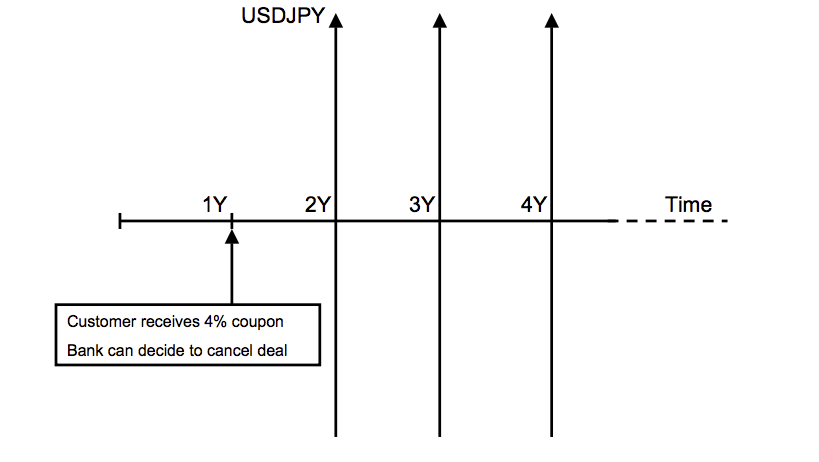
\includegraphics[width=0.5\textwidth]{pictures/PRDC.png}
\end{center}
In fact, the investor of JPY is hopping
\begin{enumerate}
   \item JPY can go strong (investor get more JPY)
   \item $r_{jpy}$ go strong (investor receive more coupon)
   \item $r_{usd}$ go weak (investor pay less coupon)

The math formular of this product is ($FX = JPY/USD$)
\begin{equation}
  PNL_t = max(0, \frac{FX_t}{FX_0}r_f - r_d)
\end{equation}

\end{enumerate}
